\section{Detailed Design Optical Emitting Payload} 
\label{sec:DDlaser}
\acs{LiDAR} is a remote sensing system comprising an optical emitting device, used to acquire topographic data, e.g. surface elevation gradients or ground composition by evaluating the \acs{BRDF}, considering multi-angular measurement are taken. For the generation of optical pulses, a highly efficient Nd:YAG (Neodymium-doped Yttrium Aluminum Garnet) hosted \ac{DPSLL}  is considered. Solid-State \acp{laser} have a high \acs{TRL} with relatively good properties in terms of beam quality (Q-factor), efficiency and pulse manipulation. Data products for topographical missions require that the \ac{laser} wave form be nearly pure Gaussian (known as transverse resonator mode $TEM_{00}$ (see figure \ref{gaussian_beam}), both temporally and spatially, with a uniform wave front. The digitized time of flight waveform returning provides the topographic structure \cite{nd_yag_life}. This section describes the detailed design of the optical emitting device; an excessive and interesting introduction of the physical basics behind \acs{laser} technology can be found in \cite{laserfundamentals}. 

\subsection{Principles of \textit{AlGaAs} Laser Diodes}
\label{laser_diodes}
Laser diodes are electrically pumped semiconductor \acp{laser}, in which the gain is generated by an electrical current flowing through a \textit{p-n junction} or (more frequently) a \textit{p-i-n structure} \cite{lasertech}. In such a heterostructure, excitons dynamics can occur (electrons and holes can recombine), releasing the energy portions as photons. This process can be spontaneous, but can also be stimulated by incident photons, in effect leading to optical amplification. Most higher-power \acs{laser} diodes, however, exhibit a relatively poor beam quality, combined with other non-favorable properties, such as a large beam divergence, high asymmetry of beam radius, non-homogeneous \textbf{k}-vector distribution and astigmatism (property of rays to exhibit different foci in different symmetrical planes) \cite{lasertech}. Especially considering the long distances used in \acs{LiDAR} missions, these properties degrade the potential data quantity, as well as quality. The basic diode \acs{laser} configuration can be found in figure \ref{diode_laser_configuration} on page \pageref{diode_laser_configuration}.

\begin{figure} [ht]
\centering
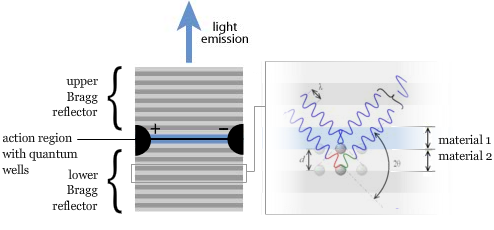
\includegraphics[scale=0.6]{chapters/img/diodelaser.png}	
\caption[Basic diode laser configuration]{Basic diode laser configuration. Each layer boundary causes a partial reflection of an optical wave. For waves whose wavelength is close to four times the optical thickness of the layers, the many reflections combine with constructive interference, and the layers act as a high-quality reflector. The range of wavelengths that are reflected is called the \textit{photonic stopband}. Bragg's law describes the condition for constructive interference from successive crystallographic planes of the crystalline lattice according to n\cdot$\lambda  =2d\cdot sin(\theta)$.} \emph{(Source: \cite{laser_power})}
\label{diode_laser_configuration}
\end{figure}

A quantum well, used in diode lasers, is a thin layer which can confine (quasi-)particles (typically electrons or holes) in the dimension perpendicular to the layer surface, whereas the movement in the other dimensions is not restricted. A quantum well is often realized with a thin layer of a semiconductor medium, embedded between other semiconductor layers of wider bandgap. The thickness of such a quantum well is typically $\sim$5 - 20 nm. 

A major challenge is to reach the laser threshold, because the optical gain for the intracavity laser beam occurs only on a very small distance (in one or several quantum wells). It is therefore necessary to realize a laser resonator with very low losses, i.e., \textit{Bragg mirrors} with high reflectivity. A Bragg mirror (also called \textit{distributed Bragg reflector}) is a structure which consists of an alternating sequence of layers of two different optical materials (see figure \ref{diode_laser_configuration}). The distance between the optical layers determines the specific photonic stopband that are optically amplified within the Bragg reflector. The presence of a spectral range has the downside, compared to discrete wavelength propagation, that the detection is less accurate, since a larger range of wavelength values should be detected and separated from noise signals. 

Individual \acs{laser} diodes normally generate quasi-continuous waves with powers $\sim$ 1 - 10 mW. To be able to generate higher power ($\sim$1 - 10 W) \textit{laser diodes arrays} or \textit{laser diode stacks} can be created, simply be combining multiple individual \acs{laser} diodes (multiple quantum wells within a diode structure). High-power \acp{LDA} are used for a variety of space-based remote sensor laser programs as an energy source for \acp{DPSSL}. \acp{LDA} have been flown on NASA missions including MOLA, GLAS and MLA and have continued to be viewed as an important part of the \acs{laser}-based instrument component suite \cite{lda_main}. 

Laser diode bars have many single emitters arranged side-by-side and spaced approximately 0.5 mm apart, on a single slab of semiconductor material measuring approximately 0.5 mm x 10 mm in size. The individual emitters are connected in parallel which keeps the required voltage low at $\sim$2 V, but increases the required current to $\sim$50 A/bar to 100 A/bar. Stacking these laser diode bars 2 to 20+ slabs high yields high power \acp{LDA} capable of emitting several hundreds of Watts. Electrically, the bars are wired in series increasing the voltage by 2 V/bar while maintaining the total current at $\sim$50 A to 100 A. These arrays are one of the enabling technologies for efficient, high power solid-state lasers.

Traditionally these arrays are operated in QCW (Quasi Continuous Wave) mode with pulse widths of $\sim$50 $\mu$s to 200 $\mu$s and repetition rates of $\sim$10 - 200 Hz. In QCW mode, the wavelength and the output power of the laser reaches steady-state, but the temperature does not. The advantage is a substantially higher output power than in CW mode, where the output power would be limited by the internal heating and the heat sinking properties of the device. The disadvantage is a much higher thermally induced mechanical stress caused by the constant heating and cooling cycle of the QCW operational mode, considering non-conductive cooling configurations.

Considering the fact that Nd:YAG is considered as gain medium (\ref{nd_yag}), the existence of strong $Nd^{3+}$ absorption near 808 nm (see figure \ref{laser})permits efficient pumping with a GaAlAs (Gallium-Aluminium-Arsenide) diode \acp{laser} for the $F_{3/2}\rightarrow I_{9/2}$ transition. The direct band gap crystal AlGaAs is often used for laser diodes with wavelengths between 750 nm and 880 nm. $Al_{x}Ga_{1-x}As$, through changing the x, the ratio of the aluminum to gallium can be adjusted to vary the band gap and thereby control the wavelength. In the double heterostructure, stimulated emission occurs only within a thin active layer of GaAs, which is sandwiched between p- and n- doped AlGaAs layers that have a wider band gap. Laser diodes use hetero junctions to achieve simultaneous carrier and photon confinement in the active region. The basic AlGaAs diode \acs{laser} configuration can be found in figure \ref{algaas_laser_configuration} on page \pageref{algaas_laser_configuration}.

\begin{figure} [ht]
\centering
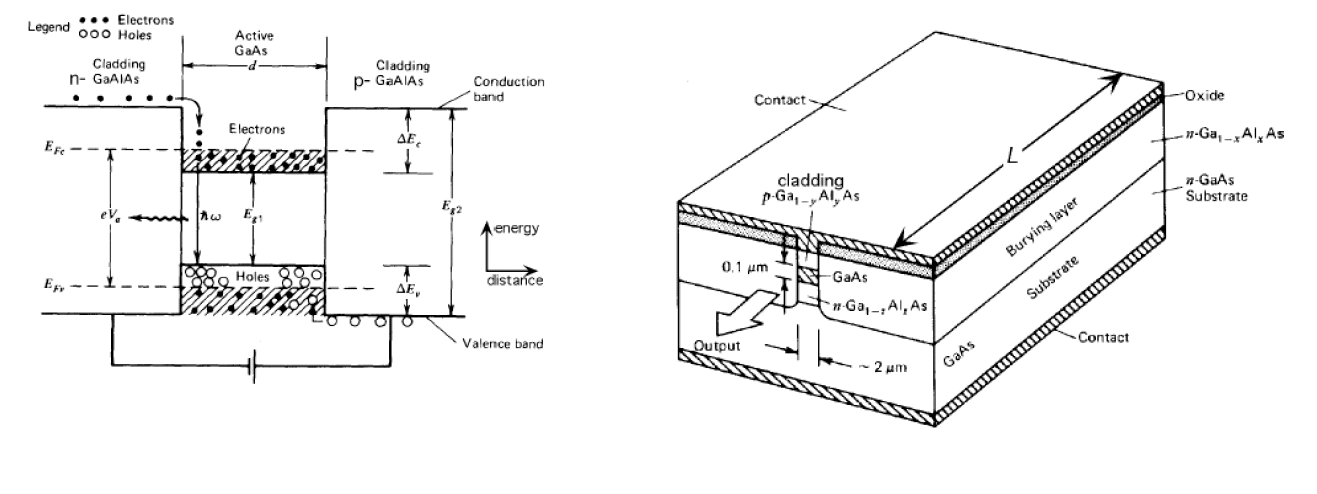
\includegraphics[scale=0.5]{chapters/img/laser_diode_algaas.png}	
\caption{AlGaAs diode laser. Left: Biased P-N junction showing elementary charge carriers. Exciton dynamics initialize after applying electrical field. Vertical direction characterizes increasing energy. Photon excitation due to stimulated emission visualized in the middle of the GaAs active layer. Right: Basic GaAs diode dimensions and components \emph{(Source: \cite{algaasdiodes})}}
\label{algaas_laser_configuration} 
\end{figure}

A high laser efficiency demands that the light and injected charge carriers be confined as closely as possible to the same volume. The AlGaAs daser diode consists of a double heterojunction formed by an undoped (or lightly p-doped) active region surrounded by high bandgap p and n $Al_{x}Ga_{1-x}As$ cladding layers \cite{algaasdiodes}. The surrounding cladding layers provide an energy barrier to confine carriers to the active region. The actual operation wavelengths may range from 750 $\sim$ 880 nm due to the effects of dopants, the size of the active region, and the compositions of the active and cladding layers. When a certain parameter is fixed, the wavelength can vary in several (sub)nanometers due to other variables. For example, when the active layer has an energy gap $E_{g} = 1.424\ eV$, the nominal emission wavelength is $\lambda = hc/E_{g}= 871\ nm$. When a bias voltage is applied in the forward direction, electrons and holes are injected into the active layer. Since the band gap energy is larger in the cladding layers than in the active layer, the injected electrons and holes are prevented from diffusing across the junction by the potential barriers formed between the active layer and cladding layers. The electrons and holes confined to the active layer create a state of population inversion, allowing the amplification of light by stimulated emission. The typical diode laser characteristics can be found in figure \ref{diode_laser_char} on page \pageref{diode_laser_char}.

\begin{figure} [ht]
\centering
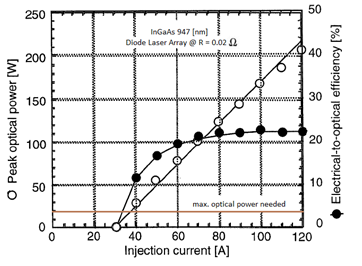
\includegraphics[scale=0.5]{chapters/img/laser_power.png}	
\caption{Typical diode \acs{laser} characteristics (P-I, \eta-I and I-U graphs). Power and current information at constant temperature. Parameters decrease with higher temperatures. Properties at desired power output (16 W): 16 A, 0.3 V, 47\%\eta}
\label{diode_laser_char}
\end{figure}

\subsection{Diode Pumped Solid-State Laser Configuration} 
\label{laserconfig}

The basic (simplified) configuration of the \acs{laser} with dimensions is shown in figure \ref{laser_dimension} on page \pageref{laser_dimension}. Individual components will be explained later in this section.

\begin{figure} [ht]
\centering
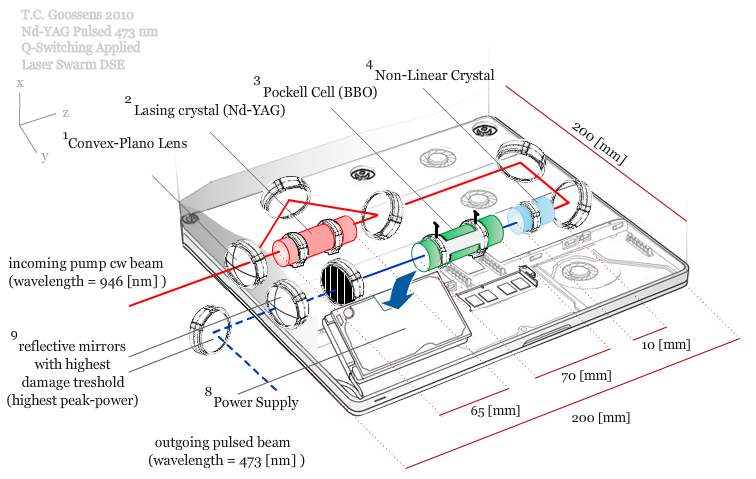
\includegraphics[scale=0.5]{chapters/img/laserconfig.png}	
\caption{Basic (simplyfied) configuration of the \acs{laser} with dimensions.}
\label{laser_dimension}
\end{figure}

\subsubsection{Nd:YAG Laser Characteristics}
\label{nd_yag}
\textit{Yttrium Aluminum Garnet} has emerged as the most widely produced laser gain host and has enjoyed recent popularity as a substrate material for optical components. The YAG host is a stable compound, mechanically robust, physically hard, optically isotropic, and transparent from below 300 to beyond 4,000 nm. YAG single crystals are able to accept trivalent laser activator ions from both the rare Earth and transition metal groups, and can be grown with very low strain. The table \ref{tab:ndyag_parameters} on page \pageref{tab:ndyag_parameters} gives the parameters of the Nd-YAG laser.

\begin{table}[ht!]
\centering
\begin{tabular}{|l|c|}
\hline
  \multicolumn{2}{|c|}{Nd-YAG (Neodymium Yttrium Aluminum Garnet $Y_3Al_5O_{12}$)}\\\hline
  Nd Concentration & 0.2 - 1.4 \% \\
  Diameter & 0.5 - 15.0 mm \\
  Length & 1.0 - 220.0 mm \\
  Damage Threshold & $> 20\ J/cm^2$  \\
  Refractive Index(n) & 1.8169 \@ 1,064 nm \\
  Thermal & 0.129 W/cm.K \\
  Conductivity & \\
  Specific Heat & 0.59 J/g.K\\
  Density & 4.55 $gm/cm^2$\\
  Tensile Strength & 280 MPa \\
  Young's Modulus & 282 GPa\\
  dn/dT & $+8.9\cdot10^{-6}\ K^{-1}$\\\hline
\end{tabular}
\caption{Solid-State laser Nd:YAG parameters}
\label{tab:ndyag_parameters}
\end{table}

For applications where $TEM_{00}$ single mode operation is required, it is necessary to reduce or eliminate the variations in the bulk material and in the absorption of the pumping radiation throughout the component. In addition, wavefront distortions due to geometric imperfections and thermal gradient effects such as thermal lensing must be minimized. In this case, Neodymium concentration in the 0.4 to 0.8\% range is typically specified.

\begin{figure} [ht]
\centering
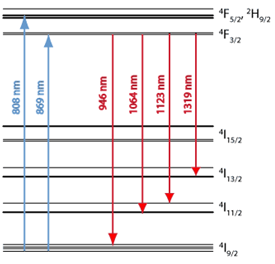
\includegraphics[scale=1.2]{chapters/img/laser_line.png}	
\caption{Left: Nd ion spectral absorption. Right: Quantum energy level and transitions for the Nd:YAG crystal, including the used $F_{3/2}\rightarrow I_{9/2}$ transition. }
\label{laser}
\end{figure}

\subsubsection{Second Harmonic Generation}
\label{SHG}
Since Nd-YAG has no principle absorption peak at the desired wavelength for the \acs{LiDAR} mission, the frequency should be altered from the original 946 nm. This can be done using \textit{second harmonic generation} or \textit{frequency doubling} in nonlinear $\beta-BaB_{2}O_{4}$ crystals.The physical mechanism behind frequency doubling can be understood using nonlinear optics \cite{laser}. Due to the first order nonlinearity, the fundamental (pump) wave generates a nonlinear polarization wave which oscillates with twice the fundamental frequency. According to Maxwell's equations, this nonlinear polarization wave radiates an electromagnetic field with this doubled frequency. Due to non-homogeneous phase-matching, the generated second-harmonic field propagates dominantly in the direction of the nonlinear polarization wave \cite(algaasdiodes); energy is transferred from the pump wave to the second-harmonic wave. $\beta-BaB_{2}O_{4}$ is used for second, third, fourth and fifth harmonic generation of Nd doping \acp{laser}. Typical dimensions of these crystal are $\sim0.05 - 10\ mm$.

\subsubsection{Pulse Generation}
\label{pockel}
The generation and manipulation of pulses can highly influent the data in \acs{LiDAR} missions. To be able to transform the quasi-continuous wave into a pulsed wave, Q-switching is applied. Q-switching is a technique for obtaining energetic short pulses from a \acs{laser} by modulating the intracavity losses and thus the Q-factor (a measure of the damping of resonator modes) of the laser resonator. The technique is mainly applied for the generation of nanosecond pulses of high energy and peak power with solid-state bulk lasers. For \textit{active Q-switching}, the losses are modulated with an active control element typically either an acousto-optic or electro-optic modulator. Both techniques rely on the fact that the optical properties within a nonlinear crystal on the occurrence of an induced sound wave (acousto-optic) or electric field (electro-optic). There are also mechanical, less viable for space missions, Q-switches such as spinning mirrors, used as end mirrors of laser resonators. In any case, the achieved pulse energy and pulse duration depends on the energy stored in the gain medium, i.e. on the pump power and the pulse repetition rate.  A Pockels cell is a device consisting of an electro-optic crystal including electrodes through which a electromagnetic beam can propagate. Dependent on the configuration, the phase delay or polarization state in the crystal (due to the \textit{Pockels effect}) can be modulated by applying a flux electric voltage (typical second harmonic generation characteristics: $\sim40,000\ V / 0.1\ mA$)  Hence, for short periods (dt) the polarization state of the incoming electromagnetic radiation can be altered. If a \textit{polarizer disk} is used after the Pockel cell, the generation of pulses will begin, since the polarizer disk transmits certain polarized states only, deflecting the rest (acting like a 'polarize filter'). Pulses in the order of nanoseconds could be created this way. Care should be taken at the fact that the peak power after the Pockel cell is increased in several orders, due to the conversion from continuous to pulsed waves. Hence, the polarizer disk should be able to cope with these stresses. According to data posted after the GLAS-mission (using the same sort of \acs{laser}, an optical induced layer was formed at the non-linear crystal, probably induced by the high peak powers of the pulsed waves. In this configuration, the pulsed wave is created after the $\beta-BaB_{2}O_{4}$ - crystal, reducing the risk of the creation of critical optical damage (COD). The figure \ref{fig:pockel_cell} on page \pageref{fig:pockel_cell} is the change in polarized state of electromagnetic radiation when passed through a Pockel cell.

\begin{figure} [ht]
\centering
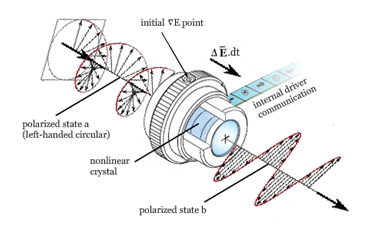
\includegraphics[scale=1.2]{chapters/img/laser_polarized.png}	
\caption[Polarized state passed through a Pockel cell]{Change in polarized state of electromagnetic radiation when passed through a Pockel cell. Communication with Pockel cell driver should be applied to determine magnitude of electric field flux and \textit{dt}. Considering the fact that the value of $f_{rep}$ could be changed in-mission (for example, if the pulse rate should be higher due to lower reflectivity on specific areas) communication with ground-station should be applied.}
\label{fig:pockel_cell}
\end{figure}

\subsection{Optical Characteristics} 
\label{opticalchar}
Considering for a moment, the radius of the beam equals 4,000 $\mu$m (due to diffraction limits, see \ref{diffraction}). Assuming a $TEM_{00}$ transverse mode of electromagnetic radiation this results in a area equal to 
\begin{equation}
\label{area}
A_{beam} = \pi \cdot r^{2} = \pi \cdot 4,000^{2} = 5,026,548\ \mu m^{2} = 0.50265\ cm^{2}
\end{equation}

The pulse energy $E_{p}$ [J] (maximum optical power of a pulse) is determined using the simulator. Sufficient energy should be present within the electromagnetic radiation to ensure the optimum path from the transmitter towards the receiver. Lowering the value of $E_{p}$ below this threshold energy can lead to atmospheric and surface absorption or translational mismatching due to incorrect scattering. The value of $E_{p}$ of this particular mission is determined to be $\sim$1 mJ (see chapter \ref{chap:sim}).
The pulse repetition rate $f_{rep}$ [Hz], i.e. the number of pulses emitted per second, is an important parameter for the altimetry mission. Again, using the results from the simulator, the quantity of this parameter can be determined to be $\sim$5000 Hz ($\Delta$t = 0.0002 s with a pulse duration $t_{p}$ $\sim$10 ns). Using the value of $f_{rep}$, the spatial resolution of the pulses along-track and in the nadir-direction can be calculated, considering the orbital velocity to be fixed at the determined altitude.  
\begin{equation}
\label{alongtrackres}
d_{along} = \Delta t \cdot v = 0.0002\ s \cdot 7,617\ m/s = 1.5234\ m
\end{equation}

\begin{equation}
\label{alongtracknadir}
d_{nadir} = \Delta t \cdot c = 0.0002\ s \cdot 299,792,458\ m/s = 59,958.49\ m
\end{equation}

Considering the value of $E_{p}$ to be 1 [mJ] with a $f_{rep}$ of 5,000 [Hz], the total power that should be induced within the electromagnetic wave can be calculated.
\begin{equation}
\label{outputpower}
P_{output} = E_{p} \cdot f_{rep} = 0.001\ J \cdot 5,000\ 1/s = 5.0\ W
\end{equation}

The \textit{total} electrical-to-optical power efficiency of a laser system ($\eta_{wp}$), i.e. the \textit{wall plug efficiency}, typically is $\sim 10\ \%$, however, linear interpolations of the current data, considering the large amount of research done on this subject, shows that $\eta_{wp}$ increases with one percent point every year (on average) from 2004, giving an wall plug efficiency of $\sim16\ \%$ in 2010 and \textgreater20 \% in 2015 \cite{nd_yag_life}. A higher value of $\eta_{wp}$ reduces the electrical power consumption and also the amount of heat which has to be removed. Simulation shows a power needed for succesfull photon detection in this altimetry mission of $\sim5 W$, ending up with a total power need of 50 W ($\eta_{wp}$=0.1) or (more realistic considering launch in 2017) 25 W ($\eta_{wp}$ = 0.2). 
  
The pulse peak intensity equals $E_{p}/t_{p} = 0.001\ J / 10\cdot10^{-9}\ s = 100,000\ W$. The intensity turns out to be $\frac{E_{p}/t_{p}}{A_{beam}} = \frac{100,000\ W}{0.50265\ cm^{2}} = 198,950.6\ W/cm^{2} (0.00199\ J/cm^{2}/10ns)$. The standard damage threshold energy $E_{p,damage}$for dielectric components equals $0.5 - 10\ J/cm^{2}/10ns$. Considering the lowest value $I_{p,damage}$, hence, $0.5\ J/cm^{2}/10ns$, and converting this to the appropriate dimensions, shows the intensity created within the electromagnetic pulses should do no harm to the dielectric components. Especially the polarizer disk (with the lowest $I_{p,damage}$) is vulnerable for peak power caused by pulsed electromagnetic radiation. 

\subsection{Gaussian Beam Propagation and Diffraction}
	\label{diffraction}

\cite{fourieroptics}Collimated plane wave propagation (uniform \textbf{k}-vector distribution) in optical systems would give rise to discrete and accurate calculations. However, due to optical distortions and modifications, the \textbf{k}-vector distribution can change, hence, altering the wave propagation. This section is based on \cite{fourieroptics} and \cite{fourieroptics1}. 

\textit{Gaussian Beams}
The figure \ref{gaussian_beam} on page \pageref{gaussian_beam} shows the mathematical desription of the Gaussian beam. For the analysis of the \acs{laser} beam intensity profile, a Gaussian profile (transverse resonator mode $TEM_{00}$) is considered corrected by the $M^{2}$ factor for optical distortion. The $M^{2}$ factor is a common measure of the beam quality of a laser beam.  The electric field distribution for a Gaussian beam is represented as:

\begin{equation}
	E(r,z) = E_{0}\cdot \frac{w_{0}}{w(z)} \cdot exp\left[\frac{-r^{2}}{w(z)}\right]\cdot exp\left[-i(kz-arctan\left(\frac{z}{z_{r}}\right)+\frac{kr^{2}}{2R(z)}\right]
\end{equation}

\begin{equation}
	E(x,y,z) = exp\left[\frac{-i(kz + \psi(z)}{w(z)}\right]exp\left[\frac{-(x^{2}+y^{2})}{w^{2}(z)} - ik \frac{(x^{2}+y^{2})}{2R(z)}\right]
\end{equation}

\begin{figure} [ht]
\centering
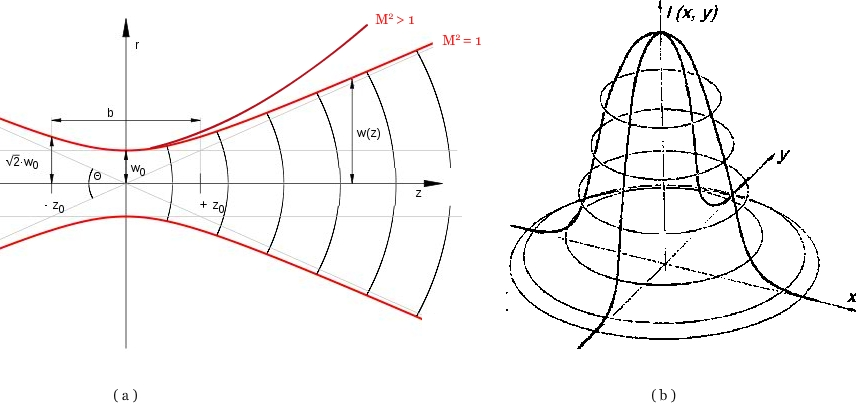
\includegraphics[scale=0.5]{chapters/img/TEM00.jpg}	
\caption{Mathematical description of the Gaussian beam/ $TEM_{00}$ transverse mode. M squared factor (negatively) influences optimum Gaussian distribution.}
\label{gaussian_beam}
\end{figure}

The main point of this section is to determine the Gaussian beam propagations dependency on diffraction phenomenon. To characterize the Gaussian beam in more details, the following equations are used to be able to describe the propagation, where \theta denotes the natural optical Gaussian beam divergence,\alpha the induced divergence (due to optical distortion and focus misalignment) and $w_{0}$ is the beam waist. 

\begin{equation}
\theta = \frac{\lambda}{\pi\cdot w_{0}}
\end{equation}

\begin{equation}
w_{real}(z)=w_{0,real}\sqrt{\left[1 + \left(\frac{z(\theta+\Delta \alpha) M^{2}}{w_{0,real}}\right)^{2}\right]}
\end{equation}

\begin{equation}
R_{real}(z)=z\left[1 + \left(\frac{w_{0,real}}{z\theta M^{2}}\right)^{2}\right]
\end{equation}

\begin{equation}
w_{real}(z)=w_{0,real}(z)\sqrt{\left[1 + \left(\frac{z\lambda M^{2}}{\pi w_{0,real}^{2}}\right)^{2}\right]}
\end{equation}

\begin{equation}
R_{real}(z)=z\left[1 + \left(\frac{w_{0,real}}{z(\theta+\Delta \alpha) M^{2}}\right)^{2}\right]
\end{equation}

\textit{Fraunhofer Diffraction} 
Diffraction is a fundamental characteristic of all wave fields. The effect of diffraction is typically manifested when an obstacle is placed (in the \acs{laser} configuration, the numerical aperture (NA) in the set-up, considering the diameter of this component equals or exceeds the \acs{laser} beam diameter) in the path of a beam.  On an observation screen some distance away from the obstacle, one observes a rather complicated modulation of the time-average intensity in the vicinity of the boundary separating the illuminated region from the geometrical shadow cast by the obstacle. With the use of high-power lasers, diffraction of radiation beams (cavity oscillating in the fundamental transverse Gaussian $TEM_{00}$ mode) with finite transverse dimensions has significant consequences. The Fresnel number $F = a^{2}/(\lambda \cdot R)$, where a is the characteristic size ("radius") of the aperture,  $\lambda$ is the wavelength, and R is the distance from the aperture, determines the diffraction regime that should be considered (F$\ll$ 1: Fraunhofer (far-field); F \textgreater 1, Fresnel). In the case of the \acs{LIDAR} mission, without actually numerically calculating the aperture, but assuming it to be \sim1 mm, the Fresnel number equals $\frac{0.001^{2}m}{(473\cdot10^{-9})m\cdot500000m}\=4.6\cdot10^{-6}$, clearly $\ll$ 1. The far-field light field is the Fourier transform of the apertured field.
	
\begin{equation} 
E(k_{x},k_{y}) = \mathcal{F}\left\{{\overbrace{t(x,y)}^{Transmission\  function}\cdot E(x,y)}\right\} = \iint(exp(-i(k_{x} x + k_{y}y))\cdot t(x,y)\cdot E(x,y)dxdy 
\end{equation}\cite{fourieroptics1} 

\begin{equation}
E(x,y,z) = \frac{exp\left[-i(kz + \psi(z))\right]}{w(z)}\cdot exp\left[\frac{-(x^{2}+y^{2})}{w^{2}(z)}-\frac{ik(x^{2}+y^{2})}{2R(z)}\right]
\end{equation}

The lens incorporates a phase delay to the outgoing electromagnetic field. For the entire derivation of the this equation, \cite{laser_power} should be evaluated (in this case, R is the curvature of the lens). 

\begin{equation}
t_{lens} = exp\left\{-i(\left((n-1)(\frac{k}{2R}(x^{2}+y^{2})\right)\right\}
\end{equation}

Combining the above calculations and using the characteristic equations for Gaussian beam properties, calculations for the Fraunhofer diffraction can be conducted, which shows the dependency on divergence.

\begin{equation}
\mathcal{F}\left\{\left(exp\left\{-i\left((n-1)\left(\frac{k}{2R(z)}\right)(x^{2}+y^{2})\right)\right\}\right)\otimes\left(\frac{exp\left[-i(kz + \psi(z))\right]}{w(z)}\cdot exp\left[\frac{-(x^{2}+y^{2})}{w^{2}(z)}-\frac{ik(x^{2}+y^{2})}{2R(z)}\right]\right)\right\}
\end{equation}\cite{fourieroptics1} 

A different point of view, conveniently in the sense of the \acs{LiDAR} mission, considers the use of focal lengths to change the Gaussian beam diffraction, giving the same result as the above Fourier transform, i.e. the divergences influence the intensity profile. The main goal of changing the divergence is influencing the footprint. Obviously, the footprints minimum size is  diffraction-limited. 

\begin{equation} 
E(x_{1},y_{1})=\iint\left[exp\left( ik\left(\frac{-2x x_{1}-2y y_{1}}{2z} + \frac{x^{2}+y^{2}}{2z}\cdot t_{lens}(x,y)\cdot E(x,y)\right)\right)\right]dx dy
\end{equation} 

Avoiding the quadratic terms and using the following relationship, the Fraunhofer diffraction pattern can be conducted \cit{fraunhoferoptics}.

\begin{equation} 
\frac{k}{2z}=(n-1)\frac{k}{2R_{1}}
\end{equation} 

Adjusting the lens formula gives:

\begin{equation} 
\frac{1}{f}=\left(n-1\right)\left[\frac{1}{R_{1}}-\frac{1}{R_{2}}\right]
\end{equation} 

The final result shows the dependency of focus length to the Fourier transform of the aperature field. 

\begin{equation} 
E(x_{1},y_{1})=\iint exp\left[-i\frac{k}{f}\left(xx_{1}+yy_{1}\right)\cdot t(x,y)\cdot E(x,y)\right] dx dy
\end{equation}


\begin{figure} [ht]
\centering
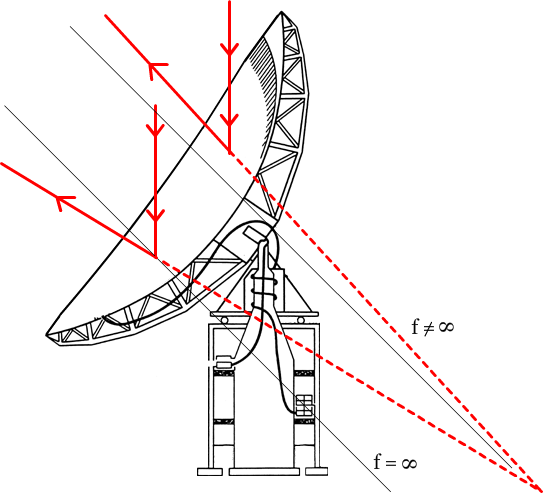
\includegraphics[scale=0.4]{chapters/img/optic_focus.png}	
\caption{Normal aligned parabolic mirror shows infinite inverse focus. Diffraction-limited case. Red lines shows induces divergence, resulting in an increase of footprint.}
\label{diff_div}
\end{figure}

Assuming infinite inverse focal length, the footprint will be diffraction limited, resulting in a footprint according to $H\cdot tan(sin^{-1}(\frac{1.22\cdot \lambda}{a}))$ \cite{fourieroptics}. With an effective aperture of 0.4 cm, the footprint due to diffraction equals 72.1325 m (96.1767 m with 0.3 cm aperture). Hence, 0.4 cm shows a considerately smaller footprint then the desired 100 m set as requirement. By altering the divergence, the footprint size can be altered. 
 
\subsection{Thermal Control} 
\label{opticalthermal}
Basically, there are three critical parts (\acs{LDA}, Nd:YAG \acs{laser} crystal and optical components after polarizer disk) of the \acs{laser} configuration in terms of thermal control. All of these components shall be considered in this subsection.

\textit{\acs{LDA}}.
The constituent parts and materials of a typical \acs{LDA} are the diode die (laser bar) and the mechanical structure. The packaging design and materials enable the array of laser bars to stay together in a stack, to be energized electrically (with a relatively high drive current), to pass the heat generated out of the unit to the mounting surface (thermal path, heat sinking), to be sufficiently rugged against mechanical insults, to provide a standard mounting interface (screws or clamps) and to be as small as possible. The active region of the \acs{LDA}, where heat is generated, is only about 1 micron wide, located about 3 microns from the P-side of the bar. The bars are about 0.1 mm wide and typically spaced about 0.5 mm from each other. Waste energy in the form of heat must be conductively transferred into the solder material and from there into the heat sink material (typically BeO or CuW) as rapidly as possible. The solder material of choice is a soft Indium alloy for its ductile property allowing the bar and the heat sink to expand or contract at different rate with temperature. The \acs{LDA} manufacturers try to use materials which possess higher thermal conductivity and a relatively comparable coefficient of thermal expansion (CTE) in order to minimize the thermal resistance of the device and the induced mechanical stresses. Additionally important to reducing mechanical stress is consideration of the use of soft solders which are highly pliable with a relatively low melting point (\~ 160 $C^{\circ}$). Post life test analysis indicates that solder deformation caused solder roll-over, in turn creating voids, which increase thermal resistance. When coupled with built-in stress due to fabrication, such roll over, in time often obstructs emitters, leading to increased heating, or extends across the bar from anode to cathode causing bar shorts which eventually result in contaminations to the emitter face and localized hot spots, further degrading performance. Excessive heating and thermal cycling of the \acs{LDA} active regions plays a key role in limiting the reliability and lifetime of \acp{LDA} operated in the QCW mode, particularly where pulse widths are long. To improve the assembles heat extraction performance, advanced materials are being considered for packaging \acp{LDA}, which have high thermal conductivity and a CTE (Coefficient of Thermal Expansion) that matches that of the laser bars to compensate inhomogeneous thermal strain. The figure \ref{thermal_control} on page \pageref{thermal_control} shows a decrease of diode lifetime as function of junction temperature.

Conductive cooling highly influences the total mass of the optical emitting payload. Normally, \acp{laser} are (partly) convection cooled using pumping cooling fluid in the neighborhood of or through the \acs{laser} components to divert waste heat. Since convection cooling is non-viable, or at least, non-preferable, in in-situ space applications, conductive cooling is applied. High powers mean high temperature gradients and hence, more conductive material. Although the configuration of the \acs{laser} differs from the HELT (\cite{nd_yag_life}), the same mass of conductive materials is considered, resulting in a total optical emitting payload mass of 15 kg. 

\begin{figure}[ht!]
\centering
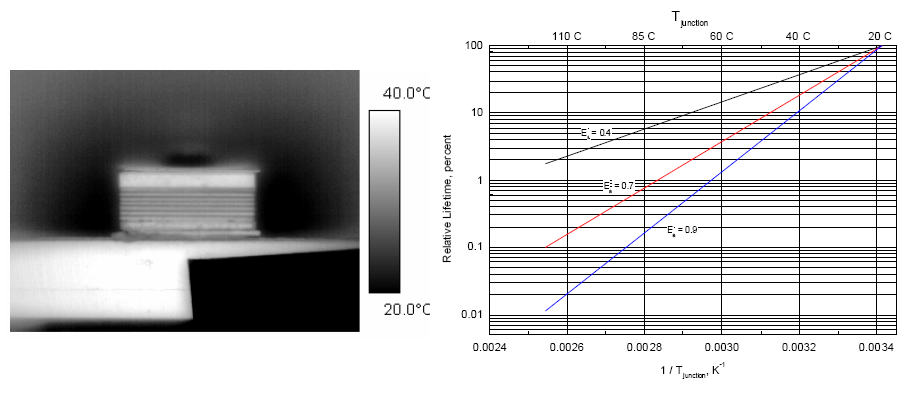
\includegraphics[scale=0.5]{chapters/img/diode_thermal.png} 
\caption{Thermal simulation of diode laser producing quasi-continuous waves (40 W, $f_{rep}$ 2,500 Hz). Graph shows a decrease of diode lifetime as function of junction temperature. \emph{(Source: \cite{thermaldiode})}}
\label{thermal_control}
\end{figure}

\textit{\acs{Nd-YAG} slab}. 
The \acs{Nd-YAG} slab plays a central role in the \acs{laser} configuration. To be able to cope with thermal stresses induced by the wave formation, the slab is thermally bonded to a molybdenum copper block in order to match the CTE.

\textit{Dilectrical Component Temperature Dependency}
Optical misalignment is a serious issue  with the \acs{laser} configuration, both in the manufacturing phase, as well during the actual mission. Refractive indices of dielectric components alter the beam translation and should be considered. Given the fact that the refractive index is a material parameter with a direct dependency of temperature (temperature-dependent Sellmeier equation), beam propagation can change unwillingly during mission. 


\subsection{ Laser Lifetime Expectancy} 
\label{opticallifetime}
Multiple aspects influence the expected lifetime of the optical emitter device, such as power, temperature interval, repetition rate and intracavity properties. Since most \acp{laser} have a non-continuous mode of operation (i.e. the duty factor is lower then 100 \%), reliability data for long-term cycles are not abundant available.  

For damage-free operation in a harsh, hands-off, environment such as space, a major form of damage risk reduction is the creation of a large single intracavity mode to reduce peak fluence. Since resonator efficiency depends strongly on the inversion density of the gain medium, it is advantageous to confine the desired cavity mode as close as possible. To accomplish this, the 808 nm light from the diode arrays should be collimated by a single plano-convex cylindrical lens (for maximal efficiency, made of undoped YAG). By doing this, the probability of the existence of thermal lensing is reduced, increasing the beam quality and the lifetime. 

Considering a constant value of $f_{rep}$ of 5,000 Hz, the total number of pulses equals $788.4\cdot10^{9}$ pulses/5 years. All optical components should be able to cope with the large amount of pulses and the peak power implied by these pulses, i.e. the energy damage threshold of the dielectric components should be higher than the incoming energy of the electromagnetic radiation. Since $I_{p,damage}$) is given with a temporal resolution in the order of a single pulse width ($\sim$10 ns), individual pulses can be analyzed. Stationary calculations can be conducted with the information based on the electromagnetic radiation energy and hence, the proper optical elements could be chosen ($I_{p,damage} > I_{p}$).

\cite{nd_yag_life} shows an experimental set-up, where the lifetime of a \acs{DPSSL} is investigated, using approximately the same \acs{laser} configuration with $f_{rep}$ = 242 Hz and $E_{p}$ = 0.0150 J. The pulse energy is much larger then the value of $E_{p}$ in the case of the \acs{LiDAR} mission described in this report ($\sim$0.001 J). Figure \ref{fig:ndyag_reliability} on page \pageref{fig:ndyag_reliability} shows the results. After $2.4\cdot10^{9}$ shots, there was no damage found in any of the cavity optics, but inspection of the diodes revealed that a single bas was lost on one array. After the first year, the pump pulse length was increased from 89 $\mu$m to 105 $\mu$m to restore the output energy to 15 mJ. This roughly simulated the procedure that would be performed in space in order to maintain an altimetry link. The final result was that after more than $4.8\cdot10^{9}$ 10 - 15 mJ laser pulses, there was no optical damage present in the system \cite{nd_yag_life}. This clearly indicates that the \acp{LDA} lifetime considerations are important for the entire \acs{laser} system. AlGaAs lasers can suffer from catastrophic optical damage (COD), rapid degradation, and gradual degradation \cite{algaas}.

\begin{figure}[ht!]
\centering
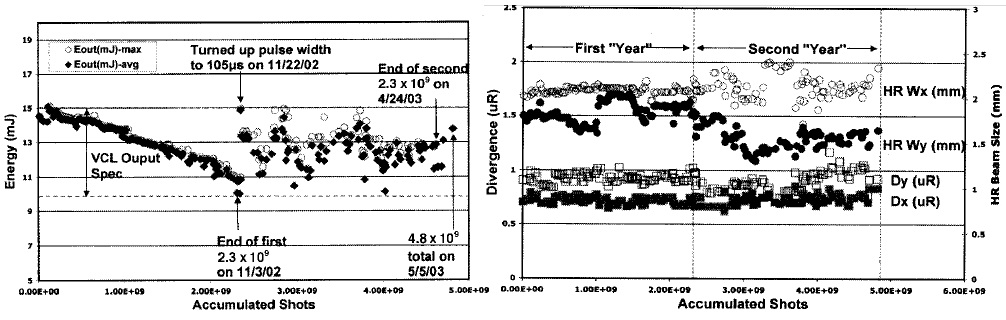
\includegraphics[scale=0.5]{chapters/img/Nd-YAG_reliability.jpg} 
\caption[Results of the conducted experiments]{Results of the conducted experiments. Results shows a steady decay in output power. After one year without any modifications, the system was reintegrated and inspected. The pulse length decrease are used to compensate for the loss in pulse power. After two years and multiple quasi-continuous shots, no optical failure occured, except single diode on the \acs{LDA} failure.}
\label{fig:ndyag_reliability}
\end{figure}

\begin{figure}[ht!]
\centering
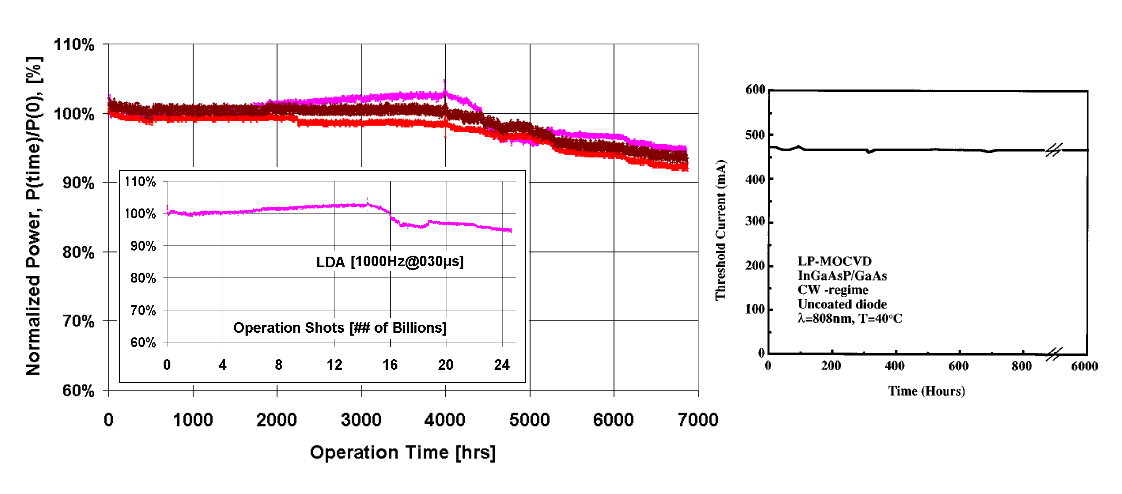
\includegraphics[scale=0.4]{chapters/img/diode_lifetime.png} 
\caption{Space-graded conductively cooled expected diode lifetime in terms of output pulses and lifetime hours (100 \% duty cycle)}.
\label{fig:diode_life_time}
\end{figure}

The figure \ref{fig:diode_life_time} on page \pageref{fig:diode_life_time} shows the space graded expected diode lifetime of the diode. Taken into account the fact that the total number of shots in five years exceed the number of total shots delivered by a single \acs{LDA} without considerable loss in power and beam quality, the obvious consequence is that multiple \acp{LDA} should be implemented within the structure. Given the fact that individual \acs{laser} diode has dimensions $\sim0.01 m$, multiple diodes could be added to form a \acs{LDA} matrix. The figure \ref{fig:laser_design_option} on page \pageref{fig:laser_design_option} gives two design options for the \acs{LDA} matrix. 

\begin{figure}[ht!]
\centering
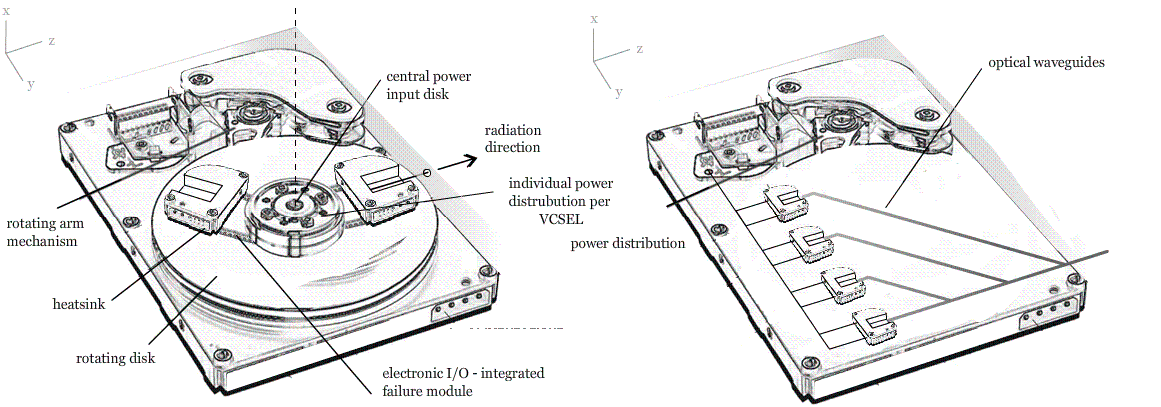
\includegraphics[scale=0.4]{chapters/img/Diode_laser.png} 
\caption[Two possible design options for the \acs{LDA} matrix]{Two possible design options for the \acs{LDA} matrix. For both cases, the individual \acp{LDA} should have communication within the subsystem, to be able to react on the failure of a single \acs{LDA}. Left: Rotating mechanism (downside: extra translation, hard to produce accurately, increased power budget), right: using optical waveguides to translate the electromagnetic radiation towards the Nd:YAG \acs{laser}}.
\label{fig:laser_design_option}
\end{figure}


\subsection{Laser Focus Calculation}
\label{focus}
The figure \ref{fig:EmitterOptics} on page \pageref{fig:EmitterOptics} gives a overview of the emitter optics. In order to diverge or focus the laser beam, it is possible to move the parabolic mirror up or down from the exact focus position. In this case, the divergent angle $\gamma$ needs to be calculated, which can be verified or optimized later on to obtain the desired footprint size. The calculation drawing is shown in figure \ref{fig:focus} on page \pageref{fig:focus}.

\begin{figure}[ht!]
\centering
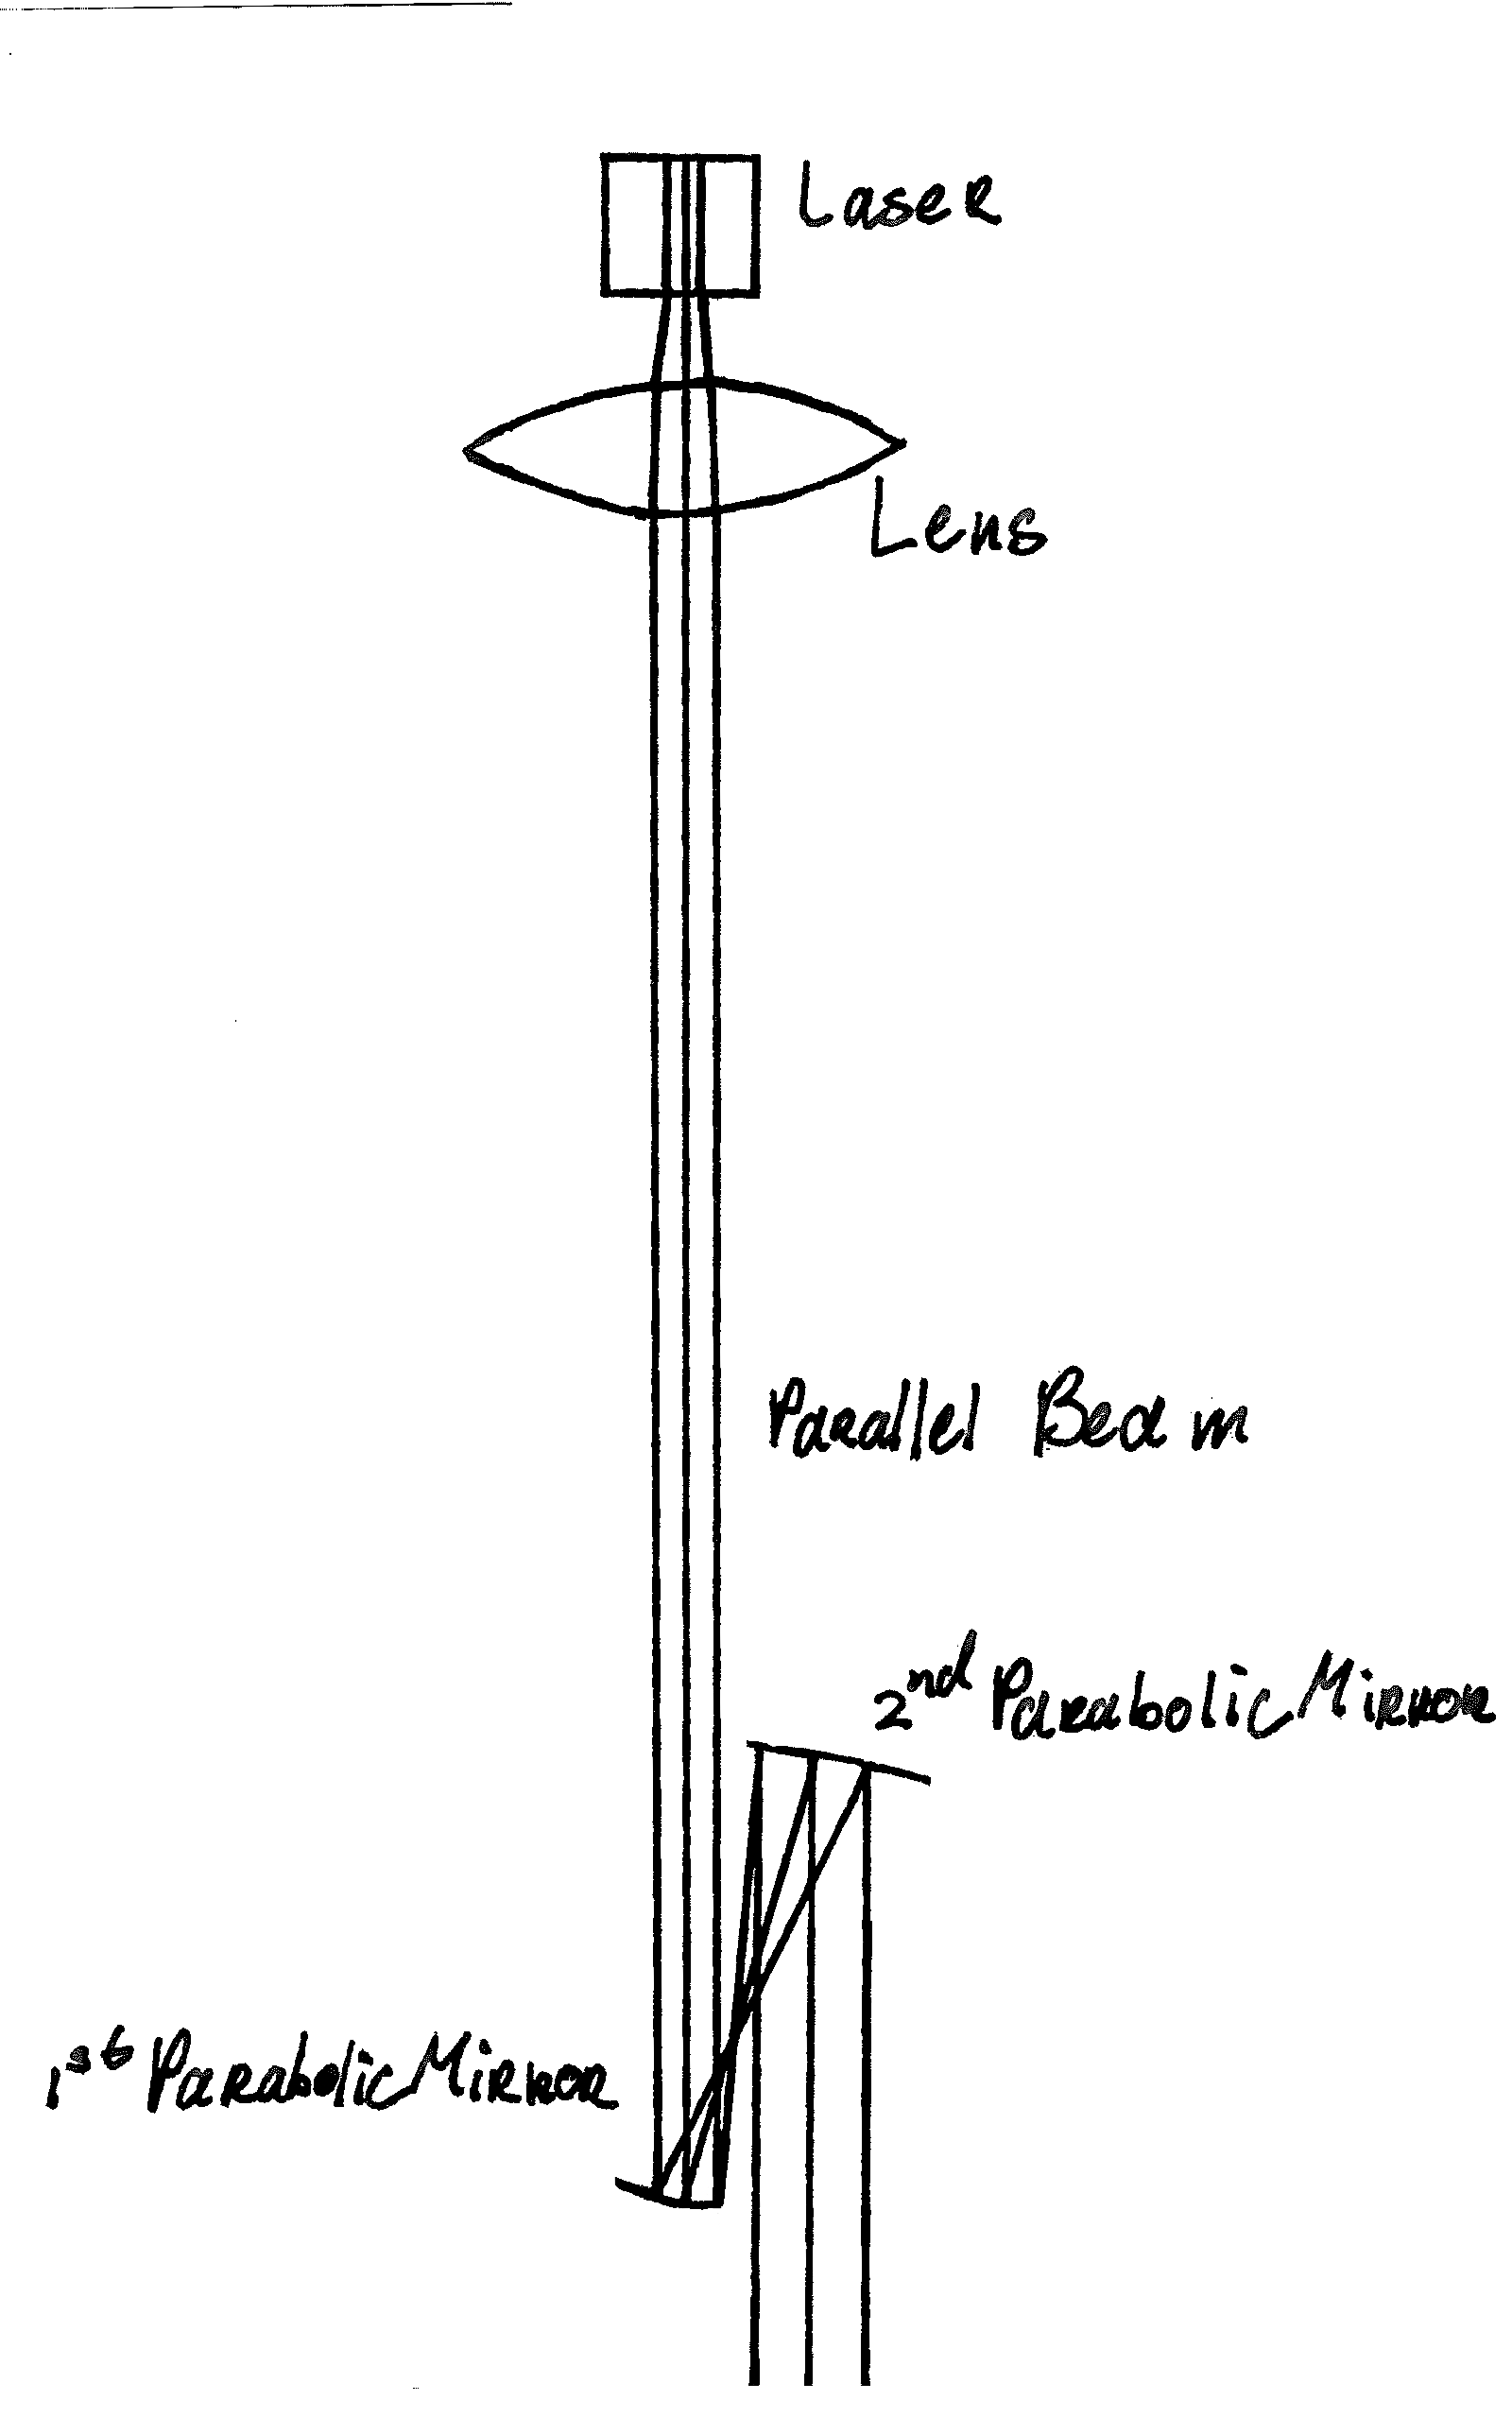
\includegraphics[scale = 0.7]{chapters/img/EmitterOptics.png}
\caption{Emitter optics drawing}
\label{fig:EmitterOptics}
\end{figure}

\begin{figure}[ht!]
\centering
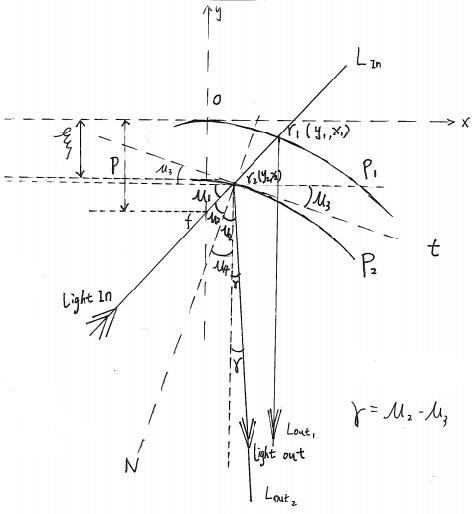
\includegraphics[scale = 1.1]{chapters/img/focus.png}
\caption{Focus calculation draft}
\label{fig:focus}
\end{figure}

In the figure \ref{fig:focus}, $p_{1}$ is the parabolic mirror positioned at the exact focus point f, and p is the distance between f and origin. $p_{2}$ is the parabolic mirror with the exact same shape but which is moved away from focus point with distance $\xi$. $L_{in}$ indicates the incoming light. $L_{out1}$ is the outcoming light due to $p_{1}$ and $L_{out2}$ is the outcoming light due to $p_{2}$. Meanwhile, $r_{1}(x_{1}, y_{1})$, $r_{2}(x_{2}, y_{2})$ are the reflected points due to $p_{1}$ and $p_{2}$. The purpose of this focusing calculation is to find the divergent angle $\gamma$ with respect to the design parameters p, $\xi$ and reflection point $r_{1}(x_{1}, y_{1}) $\cite{parabolic_wiki}. Parabolic mirror $p_{1}$ has the equation \ref{p1}, and $p_{2}$ has the equation \ref{p2}. 
\begin{equation}
\label{p1}
y = -\frac{1}{4p}x^{2}
\end {equation}
\begin{equation}
\label{p2}
y = -\frac{1}{4p}x^{2}+\xi
\end {equation}
The equation \ref{Lin} for incoming light line $L_{in}$ can be obtained since $r_{1}(x_{1}, y_{1})$ is known in this case. 
\begin{equation}
\label{Lin}
y = \frac{y_{1}+p}{x_{1}}x-p
\end {equation}
Insert equation \ref{p2} into equation \ref{Lin}, $x_{2}$ of $r_{2}(x_{2}, y_{2})$ can be obtained as:
\begin{equation}
\label{x2}
x_{2} = \frac{-\frac{y_{1}+p}{x_{1}}+\sqrt{{\frac{y_{1}+p}{x_{1}}}^2-\frac{\xi-p}{p}}}{\frac{1}{2p}}
\end {equation}
Next step is to find the tangent line of $p_{2}$ at r2:
\begin{equation}
\label{miu3}
(\frac{dy}{dx})_{x_{2}} = -\frac{1}{2p}x_{2} = tan(\mu_{3}) \Rightarrow \mu_{3} = atan(-\frac{1}{2p}x_{2})
\end {equation}
In the figure \ref{fig:focus} on page \pageref{fig:focus}, 't' is the tangent line at point $r_{2}$, and 'N' is the normal line perpendicular to the tangent line. The normal line 'N' is also the angle bisect, and $\mu_{2}$ is a half of the reflecting angle. From the drawing, these relations can be found:
\begin{equation}
\label{gamma}
\mu_{1}+\mu_{2}+\mu_{3} = 90^{\circ} = \mu_{1}+\mu_{2}+\mu_{4}
\Longrightarrow \gamma = \mu_{2} - \mu_{4} = \mu_{2} - \mu_{3} 
\end {equation}
To find $\mu_{2}$, $\mu_{1}$ need to be calculated. $\mu_{1}$ is the tangent angle of $L_{in}$ at $r_{1}$ or $r_{2}$:
\begin{equation}
\label{miu2}
(\frac{dy}{dx})_{x_{1},y_{1}} = \frac{y_{1}+p}{x_{1}} = tan(\mu{1})\Rightarrow \mu_{1} = atan(\frac{y_{1}+p}{x_{1}}) \Rightarrow \mu_{2} = 90deg - \mu_{1} - \mu_{3}
\end {equation}
Insert value of $\mu_{2}$ and $\mu_{3}$ to equation \ref{gamma}, so the divergent angle $\gamma = f(p, \xi, r_{1}(x_{1}, y_{1}))$ is obtained. Put these equations into Excel, and it is much easier to see how is $\gamma$ verified. For instance, give values for p = 350 mm, $\xi$ = 5 mm and $x_{1}$ = 5 mm, $\gamma$ = 0.01169 deg, which will give the footprint size of 102 meters. By adjusting the $\xi$, the mirror has a divergence of 20.4 m/mm for the same p and $x_{1}$.

